\documentclass{article}
\usepackage[margin=1in]{geometry}
\usepackage{amsmath,amsfonts}
\usepackage{listings}
\usepackage{fontspec}
\usepackage[bookmarks, hidelinks]{hyperref}
\usepackage{array} % For tables
\usepackage{graphicx} % 1. Include the graphicx package

% Set JetBrains Mono as the default monospaced font
\setmonofont{JetBrainsMono-Regular}

% Restore original IntelliJ-style code formatting
\lstdefinestyle{intelliJStyle}{
    language=Java,
    basicstyle=\ttfamily\small,
    numbers=left,
    numberstyle=\tiny,
    stepnumber=1,
    numbersep=5pt,
    frame=single,
    breaklines=true,
    breakatwhitespace=true,
    tabsize=1,
    showstringspaces=false,
    captionpos=b
}
\lstset{style=intelliJStyle}

\lstdefinelanguage{JavaScript}{
	keywords={
		break, case, catch, class, const, continue, debugger, default, delete, do, 
		else, export, extends, finally, for, function, if, import, in, instanceof, 
		new, return, super, switch, this, throw, try, typeof, var, void, while, with, 
		yield, static, async, await, enum, implements, interface, let, package, private, 
		protected, public, arguments
	},
	morestring=[b]",
	morestring=[b]',
	morestring=[b]\`, % Template literal support
	comment=[l]//,
	comment=[s]{/*}{*/},
	ndkeywords={
		Array, Boolean, Date, Error, EvalError, Function, Infinity, JSON, Math, NaN, 
		Number, Object, Promise, Proxy, Reflect, RegExp, Set, String, Symbol, 
		TypeError, URIError, WeakMap, WeakSet, undefined, null, console, window, 
		document, alert, setTimeout, setInterval, clearTimeout, clearInterval, 
		fetch, require, module, process
	},
	keywordstyle=\bfseries, % Keywords will be bold
	ndkeywordstyle=\slshape, % Non-declared keywords will be slanted/italic
	stringstyle=\ttfamily, % Strings will be monospaced (typewriter) font
	commentstyle=\itshape\small, % Comments will be italic and slightly smaller
	identifierstyle=, % Default style for identifiers (usually regular text)
	sensitive=true
}

% Restore original Maple language definition
\lstdefinelanguage{Maple}{
    sensitive=true,
    morecomment=[l]{--},
    morecomment=[s]{/*}{*/},
    morestring=[b]",
    morestring=[b]',
    morekeywords={and,assuming,do,else,end,export,finally,for,if,implies,in,local,module,next,not,option,or,proc,quit,read,return,save,then,use,while},
    morekeywords=[2]{array,begin,by,case,description,elif,except,fi,proc,od,otherwise,repeat,return,select,then,until,when,where},
    morekeywords=[3]{diff,int,factor,integrate,limit,signum,sum},
    alsoletter={\$},
    literate=
        {>}{{\textgreater}}1
        {<}{{\textless}}1
}

\usepackage{titlesec}
\newcommand{\sectionbreak}{\clearpage}

\usepackage{float}

\begin{document}
\bibliographystyle{plain}

\title{Fibonacci Numbers: A Deep Dive (beta)}
\author{Stanislav Ostapenko}
\date{\today}
\maketitle

\begin{abstract}
This article explores the Fibonacci sequence from basic implementations to advanced mathematical techniques. We begin with a naive recursive method, highlighting its exponential complexity and stack limitations in Java. Using a C++ JVMTI agent, we analyze JVM stack frames to understand StackOverflowException. We address Java's \texttt{long} type limitations with BigDecimal for large numbers. Optimization techniques like memoization and dynamic programming are introduced to improve performance. We derive Binet's formula using formal power series and explore matrix exponentiation for logarithmic-time computation. Finally, we discuss real-world applications, including the golden ratio, algorithms, and financial modeling.
\end{abstract}

\clearpage

	\tableofcontents % Generate table of contents

	\clearpage
	
	\lstlistoflistings % Generate list of listings

\clearpage % or \newpage

\clearpage

	\thispagestyle{empty}

	\vspace*{\fill}
	\begin{center}
		\Huge
		\begin{align*}
			&   \mathcal{O}(1) &&= \mathcal{O}(\text{yeah})\\
			&    \mathcal{O}(\log_{} n) &&= \mathcal{O}(\text{nice})\\
			&    \mathcal{O}(n) &&= \mathcal{O}(\text{k})\\
			&    \mathcal{O}(n^{2}) &&= \mathcal{O}(\text{my})\\
			&    \mathcal{O}(2^{n}) &&= \mathcal{O}(\text{no})\\
			&    \mathcal{O}(n!) &&= \mathcal{O}(\text{mg})\\
			&    \mathcal{O}(n^{n}) &&= \mathcal{O}(\text{sh*t!})
		\end{align*}
	\end{center}
	\vspace*{\fill}


\clearpage % or \newpage

\section{Recursion and Mathematical Induction}
The Fibonacci sequence, defined as $F_n = F_{n-1} + F_{n-2}$ with $F_0 = 0$ and $F_1 = 1$, is a fundamental concept in mathematics and computer science. Introduced by Leonardo of Pisa in 1202, it appears in nature (e.g., spiral patterns), algorithms (e.g., Fibonacci heaps), and number theory. We'll start our journey from naive recursion to advanced techniques, analyzing their computational complexity and practical limitations.

The concepts of recursion and mathematical induction are closely intertwined, as both rely on solving problems by breaking them down into smaller instances and establishing a base case. Below, we explore their relationship through their structural similarities and shared principles, with a particular emphasis on the role of the base case.

In mathematical induction, the base case establishes the truth of a statement for an initial value. In recursion, the base case is equally critical, as it defines the condition under which the recursive process terminates, returning a specific value without further recursive calls. The base case prevents infinite recursion and provides a foundation for building solutions to larger instances. Without a well-defined base case, a recursive function would continue indefinitely, leading to errors such as stack overflow.

For example, in a recursive factorial function, the base case is typically defined for \( n = 0 \) or \( n = 1 \), returning 1. This ensures that the recursion stops at a known value, allowing the algorithm to compute results for larger inputs by building on this foundation.

The base case is the cornerstone of both recursion and mathematical induction:
\begin{itemize}
	\item \textbf{Termination}: In recursion, the base case ensures the process stops, preventing infinite recursion. Without it, the function would attempt to compute values for invalid inputs (e.g., negative numbers) or never terminate.
	\item \textbf{Correctness}: The base case aligns with the mathematical definition of the problem, ensuring accurate results. For factorial, \( 0! = 1 \) and \( 1! = 1 \) are standard definitions.
	\item \textbf{Foundation}: It provides a starting point that recursive calls or inductive steps rely on to build the solution or proof.
\end{itemize}

Both recursion and mathematical induction rely on the principle of breaking down a problem into simpler components:
\begin{itemize}
	\item \textbf{Mathematical induction} proves a statement for all cases by starting with a base case and using the inductive step to cover all subsequent cases.
	\item \textbf{Recursion} computes a result by solving smaller instances of the same problem, reducing it to the base case.
\end{itemize}

Recursion and mathematical induction share a fundamental approach: solving or proving something by reducing it to simpler cases, anchored by a well-defined base case. The base case is essential for termination, correctness, and providing a foundation for building solutions or proofs. While induction is a proof technique, recursion is its practical counterpart in programming, with the base case playing a pivotal role in ensuring both processes succeed.
%%%%%%%%%%%%%%%%%%%%%%%%%%%%%%%%%%%%%%%%%%%%%%%

\section{Naive Recursion}
\subsection{Algorithm in Java}
The simplest approach to compute Fibonacci numbers is recursion, following the sequence's definition.

Time Complexity: $T(n) = \mathcal{O}(2^n)$ \\
Space Complexity: $M(n) = \mathcal{O}(n)$ (due to call stack depth)

\lstinputlisting[language=Java,caption={Naive Recursive Fibonacci in Java}]{./optimizing-recursion/NaiveRecursion.java}

This method is intuitive but inefficient due to redundant calculations, forming a binary recursion tree with approximately $2^n$ nodes.

\subsection{Binet's formula}
\subsubsection{Intuitive Explanation}

Let us think of the Fibonacci sequence not as a list of numbers, but as the sequence of coefficients of a power series.  
In other words, we define a generating function
\[
F(x) = F_0 + F_1x + F_2x^2 + F_3x^3 + \cdots,
\]
where each coefficient corresponds to a Fibonacci number.  

Since the Fibonacci sequence satisfies the recurrence relation
\[
F_n = F_{n-1} + F_{n-2},
\]
we can express this recurrence in terms of $F(x)$ itself.  
To do that, consider how the series looks when multiplied by $x$ and $x^2$:

\[
\left\{
\begin{aligned}
	F(x) &= F_0 + F_1x + F_2x^2 + F_3x^3 + \cdots, \\
	xF(x) &= F_0x + F_1x^2 + F_2x^3 + F_3x^4 + \cdots, \\
	x^2F(x) &= F_0x^2 + F_1x^3 + F_2x^4 + F_3x^5 + \cdots.
\end{aligned}
\right.
\]

Now, if we take $F(x) - xF(x) - x^2F(x)$, all the shifted terms cancel out due to the recurrence relation, leaving only the initial conditions:
\[
F(x) - xF(x) - x^2F(x) = F_0 + (F_1 - F_0)x.
\]
Assuming $F_0 = 0$ and $F_1 = 1$, we obtain
\[
F(x) = \frac{x}{1 - x - x^2}.
\]

The denominator here encodes the same recurrence that defines Fibonacci numbers.  
To understand the structure of $F(x)$, we factor the quadratic polynomial:
\[
1 - x - x^2 = (1 - \varphi x)(1 - \psi x),
\]
where 
\[
\varphi = \frac{1 + \sqrt{5}}{2}, \quad \psi = \frac{1 - \sqrt{5}}{2}.
\]

By the method of partial fractions, we can decompose $F(x)$ as
\[
F(x) = \frac{A}{1 - \varphi x} + \frac{B}{1 - \psi x}.
\]

Each term now has a familiar geometric series form:
\[
\frac{1}{1 - r x} = 1 + r x + r^2x^2 + r^3x^3 + \cdots,
\]
so we can directly read off the coefficients as powers of $\varphi$ and $\psi$.  

This is why we deliberately rewrite $F(x)$ in such a form:  
it allows us to transform an abstract recurrence relation into a closed analytic expression.  
Eventually, by equating coefficients of $x^n$, we recover the celebrated Binet formula:
\[
F_n = \frac{\varphi^n - \psi^n}{\sqrt{5}}.
\]

\subsubsection{Formal Derivation}

We start from the Fibonacci recurrence
\[
F_0 = 0, \qquad F_1 = 1, \qquad F_n = F_{n-1} + F_{n-2} \quad (n \ge 2).
\]

Defining the generating function
\[
F(x) = \sum_{n=0}^{\infty} F_n x^n.
\]
Then
\[
xF(x) = \sum_{n=0}^{\infty} F_n x^{n+1}, \qquad
x^2F(x) = \sum_{n=0}^{\infty} F_n x^{n+2}.
\]

Applying the recurrence relation
\[
F(x) - xF(x) - x^2F(x)
= F_0 + (F_1 - F_0)x + \sum_{n=2}^{\infty}(F_n - F_{n-1} - F_{n-2})x^n.
\]
Since $F_n - F_{n-1} - F_{n-2} = 0$ for all $n \ge 2$, we get
\[
F(x) - xF(x) - x^2F(x) = x.
\]
Hence,
\[
F(x) = \frac{x}{1 - x - x^2}.
\]

Factorization and substitution.
Let
\[
1 - x - x^2 = (1 - \varphi x)(1 - \psi x),
\]
where
\[
\varphi = \frac{1+\sqrt{5}}{2}, \qquad
\psi = \frac{1-\sqrt{5}}{2}.
\]

Then
\[
F(x) = \frac{x}{(1 - \varphi x)(1 - \psi x)}
= A\frac{x}{1 - \varphi x} + B\frac{x}{1 - \psi x}.
\]

Solving for constants.
Multiplying both sides by $(1 - \varphi x)(1 - \psi x)$:
\[
x = A(1 - \psi x) + B(1 - \varphi x)
= (A + B) - (\psi A + \varphi B)x.
\]
Matching coefficients gives
\[
A + B = 0, \qquad \varphi B + \psi A = -1.
\]
Solving:
\[
A = \frac{1}{\varphi - \psi}, \qquad B = -\frac{1}{\varphi - \psi}.
\]

Geometric series expansion
\[
\frac{1}{1 - r x} = \sum_{n=0}^{\infty} r^n x^n.
\]
Thus,
\[
F(x)
= \frac{1}{\varphi - \psi}
\left(
\frac{x}{1 - \varphi x} - \frac{x}{1 - \psi x}
\right)
= \frac{1}{\varphi - \psi}
\sum_{n=1}^{\infty} (\varphi^n - \psi^n)x^n.
\]

Extracting coefficients.
The coefficient of $x^n$ gives
\[
F_n = \frac{\varphi^n - \psi^n}{\varphi - \psi}
= \frac{1}{\sqrt{5}}
\left[
\left(\frac{1+\sqrt{5}}{2}\right)^n
- \left(\frac{1-\sqrt{5}}{2}\right)^n
\right].
\]

\[
\boxed{
	F_n = \frac{\varphi^n - \psi^n}{\sqrt{5}}
}
\]
This is the closed form known as \textbf{Binet's formula}.


% Analyzing time complexity
\subsection{Time Complexity (Big $\mathcal{O}$)}
The recursive algorithm generates a binary recursion tree, where each node for \( n \geq 2 \) spawns two child nodes: \( F(n-1) \) and \( F(n-2) \).
The total number of function calls corresponds to the number of nodes in the recursion tree. For a given \( n \), the tree has a depth of approximately \( n \), and the number of nodes grows exponentially. The recurrence relation for the number of operations \( T(n) \) is:
\[
T(n) = T(n-1) + T(n-2) + O(1),
\]
where \( O(1) \) accounts for the constant-time addition operation. The base cases are:
\[
T(0) = O(1), \quad T(1) = O(1).
\]

This recurrence is similar to the Fibonacci sequence itself. The number of nodes is approximately \( 2F(n) - 1 \), where \( F(n) \approx \phi^n / \sqrt{5} \), and \( \phi = \frac{1 + \sqrt{5}}{2} \approx 1.618 \) is the golden ratio. Thus, the time complexity is:
\[
T(n) = O(\phi^n) \approx O(1.618^n).
\]

%%%%%%%%%%%%
\subsection{Empirical Validation of Time Complexity}
Let's calculate execution time of first 50 Fibonacci numbers. Also, save exec results in CSV file further for analysis.
\lstinputlisting[language=Java]{./recursive-time-exec/RecursiveGrowthDemonstrator.java}
To show how the time grows, let's build a chart -
\begin{figure}[H]
	\centering
	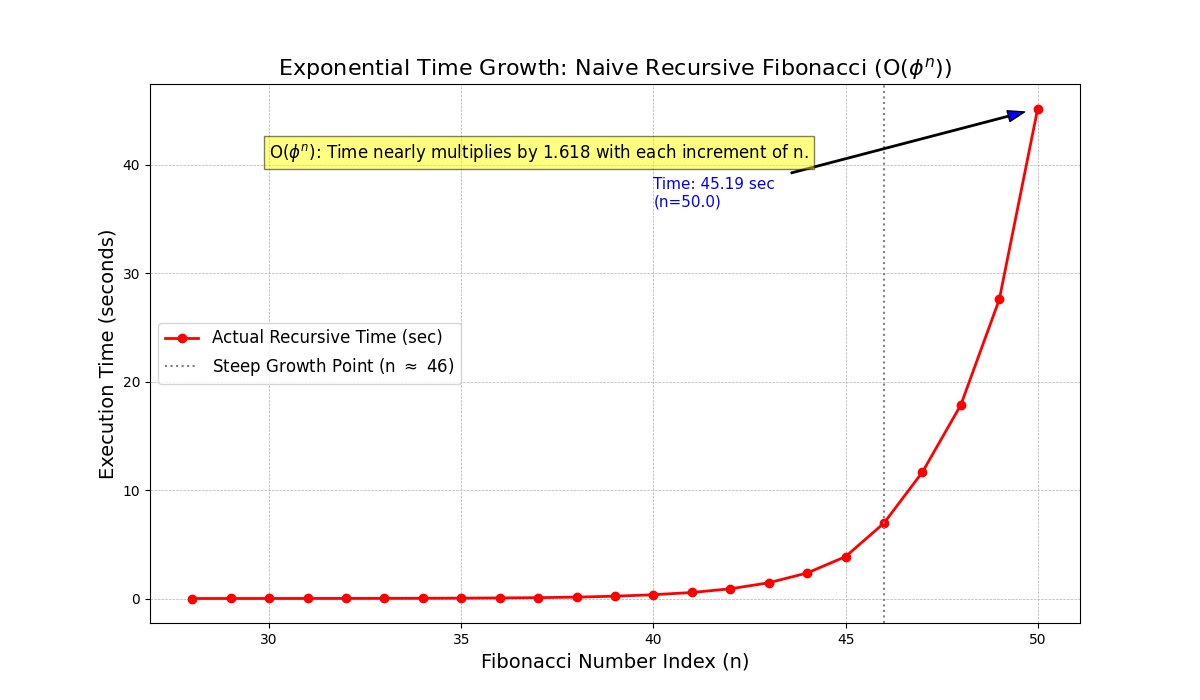
\includegraphics[width=0.9\textwidth]{./recursive-time-exec/exponential-time-growth.png}
	\caption{Exponent execution time}
	\label{fig:exponent_growth}
\end{figure}

To produce this image we use Python with some Pandas :
\lstinputlisting[language=Python]{./recursive-time-exec/fib-exec-time-chart.py}

Now we are interested in exact formula of this type of growth. To achieve our goal we'll going to use SciPy.
\lstinputlisting[language=Python]{./recursive-time-exec/empiristic-formula-for-time-complexity.py}

Which shows us the following : 
\begin{figure}[H]
	\centering
	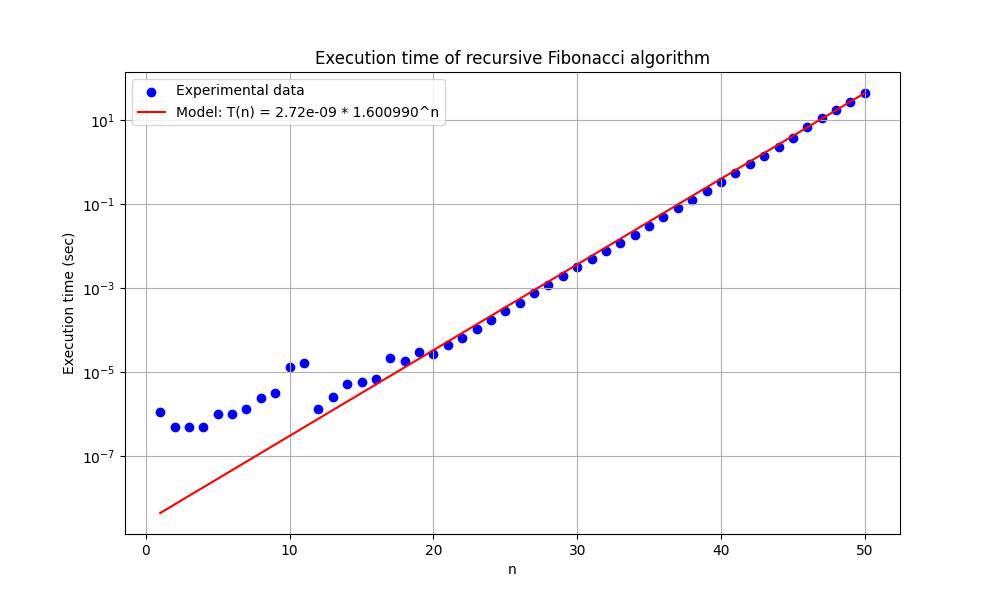
\includegraphics[width=0.9\textwidth]{./recursive-time-exec/experimental-data-formula.png}
	\caption{Exponent execution time}
	\label{fig:experimental_vs_theoretical}
\end{figure}

Axes made logarithmic for better looking chart.
So, we have result of out numerical modeling 
\begin{lstlisting}[language=bash]
python empiristic-formula-for-time-complexity.py
Fitted model: T(n) = 0.0000000027 * 1.600990^n
Golden ratio (φ): 1.618034
Deviation of b from φ: 0.017044
\end{lstlisting}
%%%%%%%%%%%%

So, we can have exec time needed to calculate n-th fib. It grows fast and could be very big.

\begin{table}[h]
	\centering
	\caption{Estimated execution time of recursive Fibonacci algorithm using the model $T(n) = 2.7 \times 10^{-9} \cdot 1.600990^n$}
	\begin{tabular}{|c|c|c|}
		\hline
		$n$ & $T(n)$ & Unit \\
		\hline
		20 & 3.30e-05 & sec \\ 
		\hline
		30 & 3.66e-03 & sec \\ 
		\hline
		40 & 4.04e-01 & sec \\ 
		\hline
		50 & 4.48e+01 & sec \\ 
		\hline
		60 & 1.3752 & hr \\ 
		\hline
		70 & 6.3395 & days \\ 
		\hline
		80 & 1.9215 & yr \\ 
		\hline
		90 & 212.5851 & yr \\ 
		\hline
		100 & 23519.0125 & yr \\ 
		\hline
		
	\end{tabular}
\end{table}

So, we have kind of bad news here. To calculate $F(100)$ we'll need $\approx 25 000$ years. Too long to wait, soon we improve algorithm.

% Creating a section for JVM Memory Structures
\subsection{Introduction to JVM Memory Structures}

% Introducing the JVM and its memory architecture
The Java Virtual Machine (JVM) is a runtime environment that executes Java bytecode, enabling platform-independent execution of Java programs. The JVM manages memory through a structured architecture that supports dynamic allocation, thread execution, and garbage collection.

% Subsection for overview of JVM memory

The JVM divides its memory into several regions, each serving a specific purpose in program execution. These regions are broadly categorized into \textbf{per-thread} and \textbf{shared} areas:
\begin{itemize}
	\item \textbf{Per-Thread Areas}: Allocated for each thread to ensure isolation and manage method execution.
	\item \textbf{Shared Areas}: Accessible by all threads for storing objects and class metadata.
\end{itemize}
Memory management is critical for performance, as it affects allocation speed, garbage collection, and thread synchronization. The JVM's memory model is defined by the Java Virtual Machine Specification (JVMS).

The JVM's memory is organized into the following key areas:
\begin{enumerate}
	\item \textbf{Heap}:
	\begin{itemize}
		\item A shared memory region where all objects and arrays are allocated using the \texttt{new} keyword.
		\item Divided into:
		\begin{itemize}
			\item \textbf{Young Generation} (Eden and Survivor spaces): For newly created objects, managed by frequent minor garbage collections.
			\item \textbf{Old Generation}: For long-lived objects, managed by less frequent major garbage collections.
			\item \textbf{Metaspace} (Java 8+): Stores class metadata, replacing the Permanent Generation (pre-Java 8).
		\end{itemize}
		\item Configurable via flags like \texttt{-Xmx} (maximum heap size) and \texttt{-Xms} (initial heap size).
	\end{itemize}
	\item \textbf{Java Stack}:
	\begin{itemize}
		\item A per-thread memory area that stores \textbf{call frames} for method invocations.
		\item Each frame contains a local variable array, operand stack, and frame data (e.g., program counter, return address).
		\item Size is configurable via \texttt{-Xss}. Excessive recursion can cause a \texttt{StackOverflowError}.
	\end{itemize}
	\item \textbf{Program Counter (PC) Register}:
	\begin{itemize}
		\item A per-thread register that holds the address of the current bytecode instruction being executed.
		\item Points to the current instruction in the active call frame's bytecode.
	\end{itemize}
	\item \textbf{Method Area}:
	\begin{itemize}
		\item A shared area that stores class metadata, including bytecode, constant pools, and method tables.
		\item In Java 8+, the Method Area is implemented as Metaspace, which uses native memory rather than the heap.
	\end{itemize}
	\item \textbf{Native Method Stack}:
	\begin{itemize}
		\item A per-thread stack for executing native methods (e.g., C/C++ code called via JNI).
		\item Similar to the Java stack but tailored for non-Java code.
	\end{itemize}
\end{enumerate}

% Table summarizing memory regions
\begin{table}[h]
	\centering
	\begin{tabular}{|>{\raggedright\arraybackslash}m{3cm}|>{\raggedright\arraybackslash}m{4cm}|>{\raggedright\arraybackslash}m{5cm}|}
		\hline
		\textbf{Memory Region} & \textbf{Type} & \textbf{Purpose} \\
		\hline
		Heap & Shared & Stores objects, arrays, and class metadata (Metaspace in Java 8+) \\
		Java Stack & Per-thread & Stores call frames for method execution \\
		PC Register & Per-thread & Tracks current bytecode instruction \\
		Method Area & Shared & Stores class metadata and constant pools \\
		Native Method Stack & Per-thread & Manages native method execution \\
		\hline
	\end{tabular}
	\caption{JVM Memory Regions}
\end{table}

Consider this Java code:
\begin{lstlisting}[language=Java]
public class Example {
	public static void main(String[] args) {
		String str = new String("Hello");
		int result = add(3, 4);
		System.out.println(str + result);
	}
	public static int add(int a, int b) {
		return a + b;
	}
}
\end{lstlisting}

\begin{enumerate}
	\item \textbf{Heap}: The \texttt{String} object \texttt{"Hello"} is allocated in the heap's Eden space.
	\item \textbf{Java Stack}: The \texttt{main} method's call frame stores the \texttt{str} reference and \texttt{args}. A new frame for \texttt{add} stores parameters \texttt{a} and \texttt{b}.
	\item \textbf{PC Register}: Tracks the current bytecode instruction in \texttt{main} or \texttt{add}.
	\item \textbf{Method Area}: Stores the bytecode and constant pool for \texttt{Example} class, including the \texttt{"Hello"} string literal.
	\item \textbf{Garbage Collection}: After \texttt{main} ends, the \texttt{String} object may be reclaimed if no references remain.
\end{enumerate}

The memory structures work together to support JVM execution:
\begin{itemize}
	\item \textbf{Thread Isolation}: Per-thread areas (Java Stack, PC Register, Native Method Stack) ensure threads execute independently without interference.
	\item \textbf{Shared Resources}: The heap and Method Area (or Metaspace) allow threads to share objects and class data, requiring synchronization (e.g., \texttt{synchronized} blocks) to avoid race conditions.
	\item \textbf{Garbage Collection}: The garbage collector scans the heap, using references from stacks, Method Area, and static fields as roots to identify reachable objects.
\end{itemize}

Key Concepts :
\begin{itemize}
	\item \textbf{Heap vs. Stack}: Heap stores dynamic, shared objects; stacks store method-scoped, thread-specific data.
	\item \textbf{Garbage Collection}: Automatically reclaims heap memory but requires careful reference management to avoid leaks.
	\item \textbf{Performance}: Memory size tuning (e.g., \texttt{-Xmx}, \texttt{-Xss}) impacts performance. Large heaps or stacks may slow execution or garbage collection.
	\item \textbf{Debugging}: Tools like \texttt{jstack} (for stacks), \texttt{jmap} (for heap), and VisualVM help analyze memory usage and diagnose issues.
\end{itemize}

%%%%%%%%%%%%%%%%%%%%%
% Creating a unified section combining pass-by-value, recursion, tail recursion, TCO comparison, bytecode, and method execution
\subsection{Method Execution in Java}

\subsubsection{Core concepts}
Java’s method invocation and parameter passing mechanisms are central to understanding its runtime behavior in the Java Virtual Machine (JVM). Java exclusively uses \textbf{pass-by-value} for all parameter passing, impacting both iterative and recursive methods. Recursion, including \textbf{tail recursion}, interacts with the JVM’s stack and heap, while Java’s lack of \textbf{tail call optimization (TCO)} affects performance in deep recursion. 
\begin{itemize}
	\item \textbf{Pass-by-Value}: The method receives a copy of the argument’s value (primitive or object reference). Changes to the parameter do not affect the caller’s variable.
	\item \textbf{Pass-by-Reference}: The method receives a reference to the original argument’s memory location, so changes directly modify the caller’s variable.
\end{itemize}
Java uses \textbf{pass-by-value} exclusively. For \textbf{primitive types} (e.g., \texttt{int}, \texttt{double}), the value is copied. For \textbf{object references}, the reference (not the object) is copied, allowing modification of the object’s state in the heap but not reassignment of the caller’s reference.

% Explaining pass-by-value in Java
\subsubsection{Pass-by-Value in Java}
When a method is called, the JVM creates a call frame on the thread’s Java stack, copying arguments into the frame’s local variable array:
\begin{itemize}
	\item \textbf{Primitive Types}: The value (e.g., 5 for an \texttt{int}) is copied. Modifying the parameter changes only the local copy.
	\item \textbf{Object References}: The reference (memory address to a heap object) is copied. Modifying the object’s state (e.g., fields) affects the heap, visible to all references. Reassigning the reference (e.g., \texttt{obj = new Object()}) is local.
\end{itemize}
This behavior applies to both iterative and recursive methods, but recursion increases stack depth, risking \texttt{StackOverflowError} for deep calls.

Consider a Java program demonstrating pass-by-value in both iterative and recursive contexts:
\begin{lstlisting}
	public class Example {
		public static void main(String[] args) {
			int num = 5;
			StringBuilder sb = new StringBuilder("Factorial: ");
			modifyPrimitive(num);
			modifyObject(sb);
			int result = factorialTail(num, 1, sb);
			System.out.println("num: " + num); // Outputs: num: 5
			System.out.println("sb: " + sb + " " + result); // Outputs: sb: Factorial: 5*4*3*2*1 120
		}
		
		public static void modifyPrimitive(int x) {
			x = 10; // Modifies local copy
		}
		
		public static void modifyObject(StringBuilder builder) {
			builder.append("World"); // Modifies heap object
			builder = new StringBuilder("New"); // Local reassignment
		}
		
		public static int factorialTail(int n, int acc, StringBuilder log) {
			if (n <= 1) {
				log.append("1");
				return acc;
			}
			log.append(n + "*");
			return factorialTail(n - 1, n * acc, log); // Tail-recursive call
		}
	}
\end{lstlisting}
\begin{enumerate}
	\item \textbf{Primitive (\texttt{num})}: In \texttt{modifyPrimitive}, \texttt{x} is a copy of \texttt{num} (5). Setting \texttt{x = 10} affects only the local copy, so \texttt{num} remains 5.
	\item \textbf{Object Reference (\texttt{sb})}: In \texttt{modifyObject}, \texttt{builder} is a copy of the reference to \texttt{StringBuilder}. \texttt{builder.append("World")} modifies the heap object, affecting \texttt{sb}. Reassigning \texttt{builder = new StringBuilder("New")} is local, so \texttt{sb} retains its reference.
	\item \textbf{Tail Recursion (\texttt{factorialTail})}: Each recursive call copies \texttt{n}, \texttt{acc}, and \texttt{log}. Modifications to \texttt{log} (e.g., \texttt{log.append(n + "*")}) persist in the heap. The recursive call is the last operation, but Java creates a new frame each time, risking stack overflow for large \texttt{n}.
\end{enumerate}

% Explaining tail recursion and lack of TCO
\subsubsection{Tail Recursion}
A method is \textbf{tail-recursive} if the recursive call is the final operation, with no pending computations. In languages with \textbf{tail call optimization (TCO)}, the runtime reuses the current frame, avoiding stack growth. Java’s JVM does not support TCO, so each recursive call creates a new frame, copying arguments via pass-by-value.
It's because JVM prioritizes general-purpose execution and accurate stack traces for debugging over TCO.
\\
TCO support varies across languages, impacting recursion efficiency:
\begin{itemize}
	\item \textbf{Java}: No TCO; each call adds a frame, risking \texttt{StackOverflowError}.
	\item \textbf{Scala}: TCO for self-recursive calls with \texttt{@tailrec}, compiling to loops on the JVM.
	\item \textbf{Python}: No TCO; uses iteration or trampolining for deep recursion.
	\item \textbf{JavaScript}: Partial TCO (e.g., Safari supports it, V8 does not).
	\item \textbf{Haskell}: Full TCO with lazy evaluation, ideal for recursion-heavy code.
\end{itemize}
\begin{table}[h]
	\centering
	\begin{tabular}{|>{\raggedright\arraybackslash}m{2.5cm}|>{\raggedright\arraybackslash}m{3cm}|>{\raggedright\arraybackslash}m{3cm}|}
		\hline
		\textbf{Language} & \textbf{TCO Support} & \textbf{Workaround} \\
		\hline
		Java & None & Iteration \\
		Scala & Yes (\texttt{@tailrec}) & None needed \\
		Python & None & Iteration \\
		JavaScript & Partial & Iteration \\
		Haskell & Full & None needed \\
		\hline
	\end{tabular}
	\caption{Tail Call Optimization Across Languages}
\end{table}

%%%%%%%%%%%%%%%%%%%%%
%%\subsection{Depth and \lstinline[style=keyword]\{StackOverflow\}}
\subsection{Depth and \lstinline[basicstyle=\ttfamily\small]{StackOverflow}}
Recursive calls create stack frames in the JVM, which can lead to a \texttt{StackOverflowError}. We demonstrate this with a simple recursive program :
\lstinputlisting[language=Java,caption={Testing Recursion Depth}]{./recursion-tree/RecursionDepth.java}
Run with:
\begin{lstlisting}[language=bash,caption={Running RecursionDepth}]
	java -Xss1m RecursionDepth
\end{lstlisting}

It means that even without calculating something, we limited by the value of stack. God news is that it could be increased, but we have no clue how much we need.

%%%%%%%%%%%%%%%%%%%%%
\subsection{Recursion Tree}
%% todo
\lstinputlisting[language=Java,caption={Recursion StackTrace}]{./recursion-tree/StackTraceDepth.java}
We have to have compare depth calculation and number of frames, make conclusions.

Output : 
\begin{lstlisting}[language=bash]
> java StackTraceDepth
fib0(5) depth=1 frames=3
fib0(4) depth=2 frames=4
fib0(3) depth=3 frames=5
fib0(2) depth=4 frames=6
fib0(1) depth=5 frames=7
fib0(0) depth=5 frames=7
fib0(1) depth=4 frames=6
fib0(2) depth=3 frames=5
fib0(1) depth=4 frames=6
fib0(0) depth=4 frames=6
fib0(3) depth=2 frames=4
fib0(2) depth=3 frames=5
fib0(1) depth=4 frames=6
fib0(0) depth=4 frames=6
fib0(1) depth=3 frames=5
Result: 5
\end{lstlisting}

Let's make an improvement. We'll all ident to previous code according to depth
\lstinputlisting[language=Java,caption={Recursion indent}]{./recursion-tree/SimpleIdent.java}
\newpage
Output is better. BTW code is good for debugging any recursion.
\begin{lstlisting}[language=bash]
fib0(5) depth=0
  fib0(4) depth=1
    fib0(3) depth=2
      fib0(2) depth=3
        fib0(1) depth=4
        => fib0(1) = 1
        fib0(0) depth=4
        => fib0(0) = 0
      => fib0(2) = 1
      fib0(1) depth=3
      => fib0(1) = 1
    => fib0(3) = 2
    fib0(2) depth=2
      fib0(1) depth=3
      => fib0(1) = 1
      fib0(0) depth=3
      => fib0(0) = 0
    => fib0(2) = 1
  => fib0(4) = 3
  fib0(3) depth=1
    fib0(2) depth=2
      fib0(1) depth=3
      => fib0(1) = 1
      fib0(0) depth=3
      => fib0(0) = 0
    => fib0(2) = 1
    fib0(1) depth=2
    => fib0(1) = 1
  => fib0(3) = 2
=> fib0(5) = 5
Result: 5
\end{lstlisting}

We can do better. Let's buid a tree using dot syntax (blah-blah-blah)
\lstinputlisting[language=Java, caption={Recursion tree generator}]{./recursion-tree/RecursionGraphvizTree.java}

And here it is : 
\begin{figure}[H] % The figure environment helps with placement and captions
	\centering
	\includegraphics[width=0.8\textwidth]{./recursion-tree/fib\_tree.png}
	\caption{Recursion tree} % Caption for the image
	\label{fig:logo} % Label for cross-referencing
\end{figure}

\newpage
As you can see in Figure \ref{fig:logo}, recursion tree is displayed nicely.

Or even better
\begin{figure}[H]
	\centering
	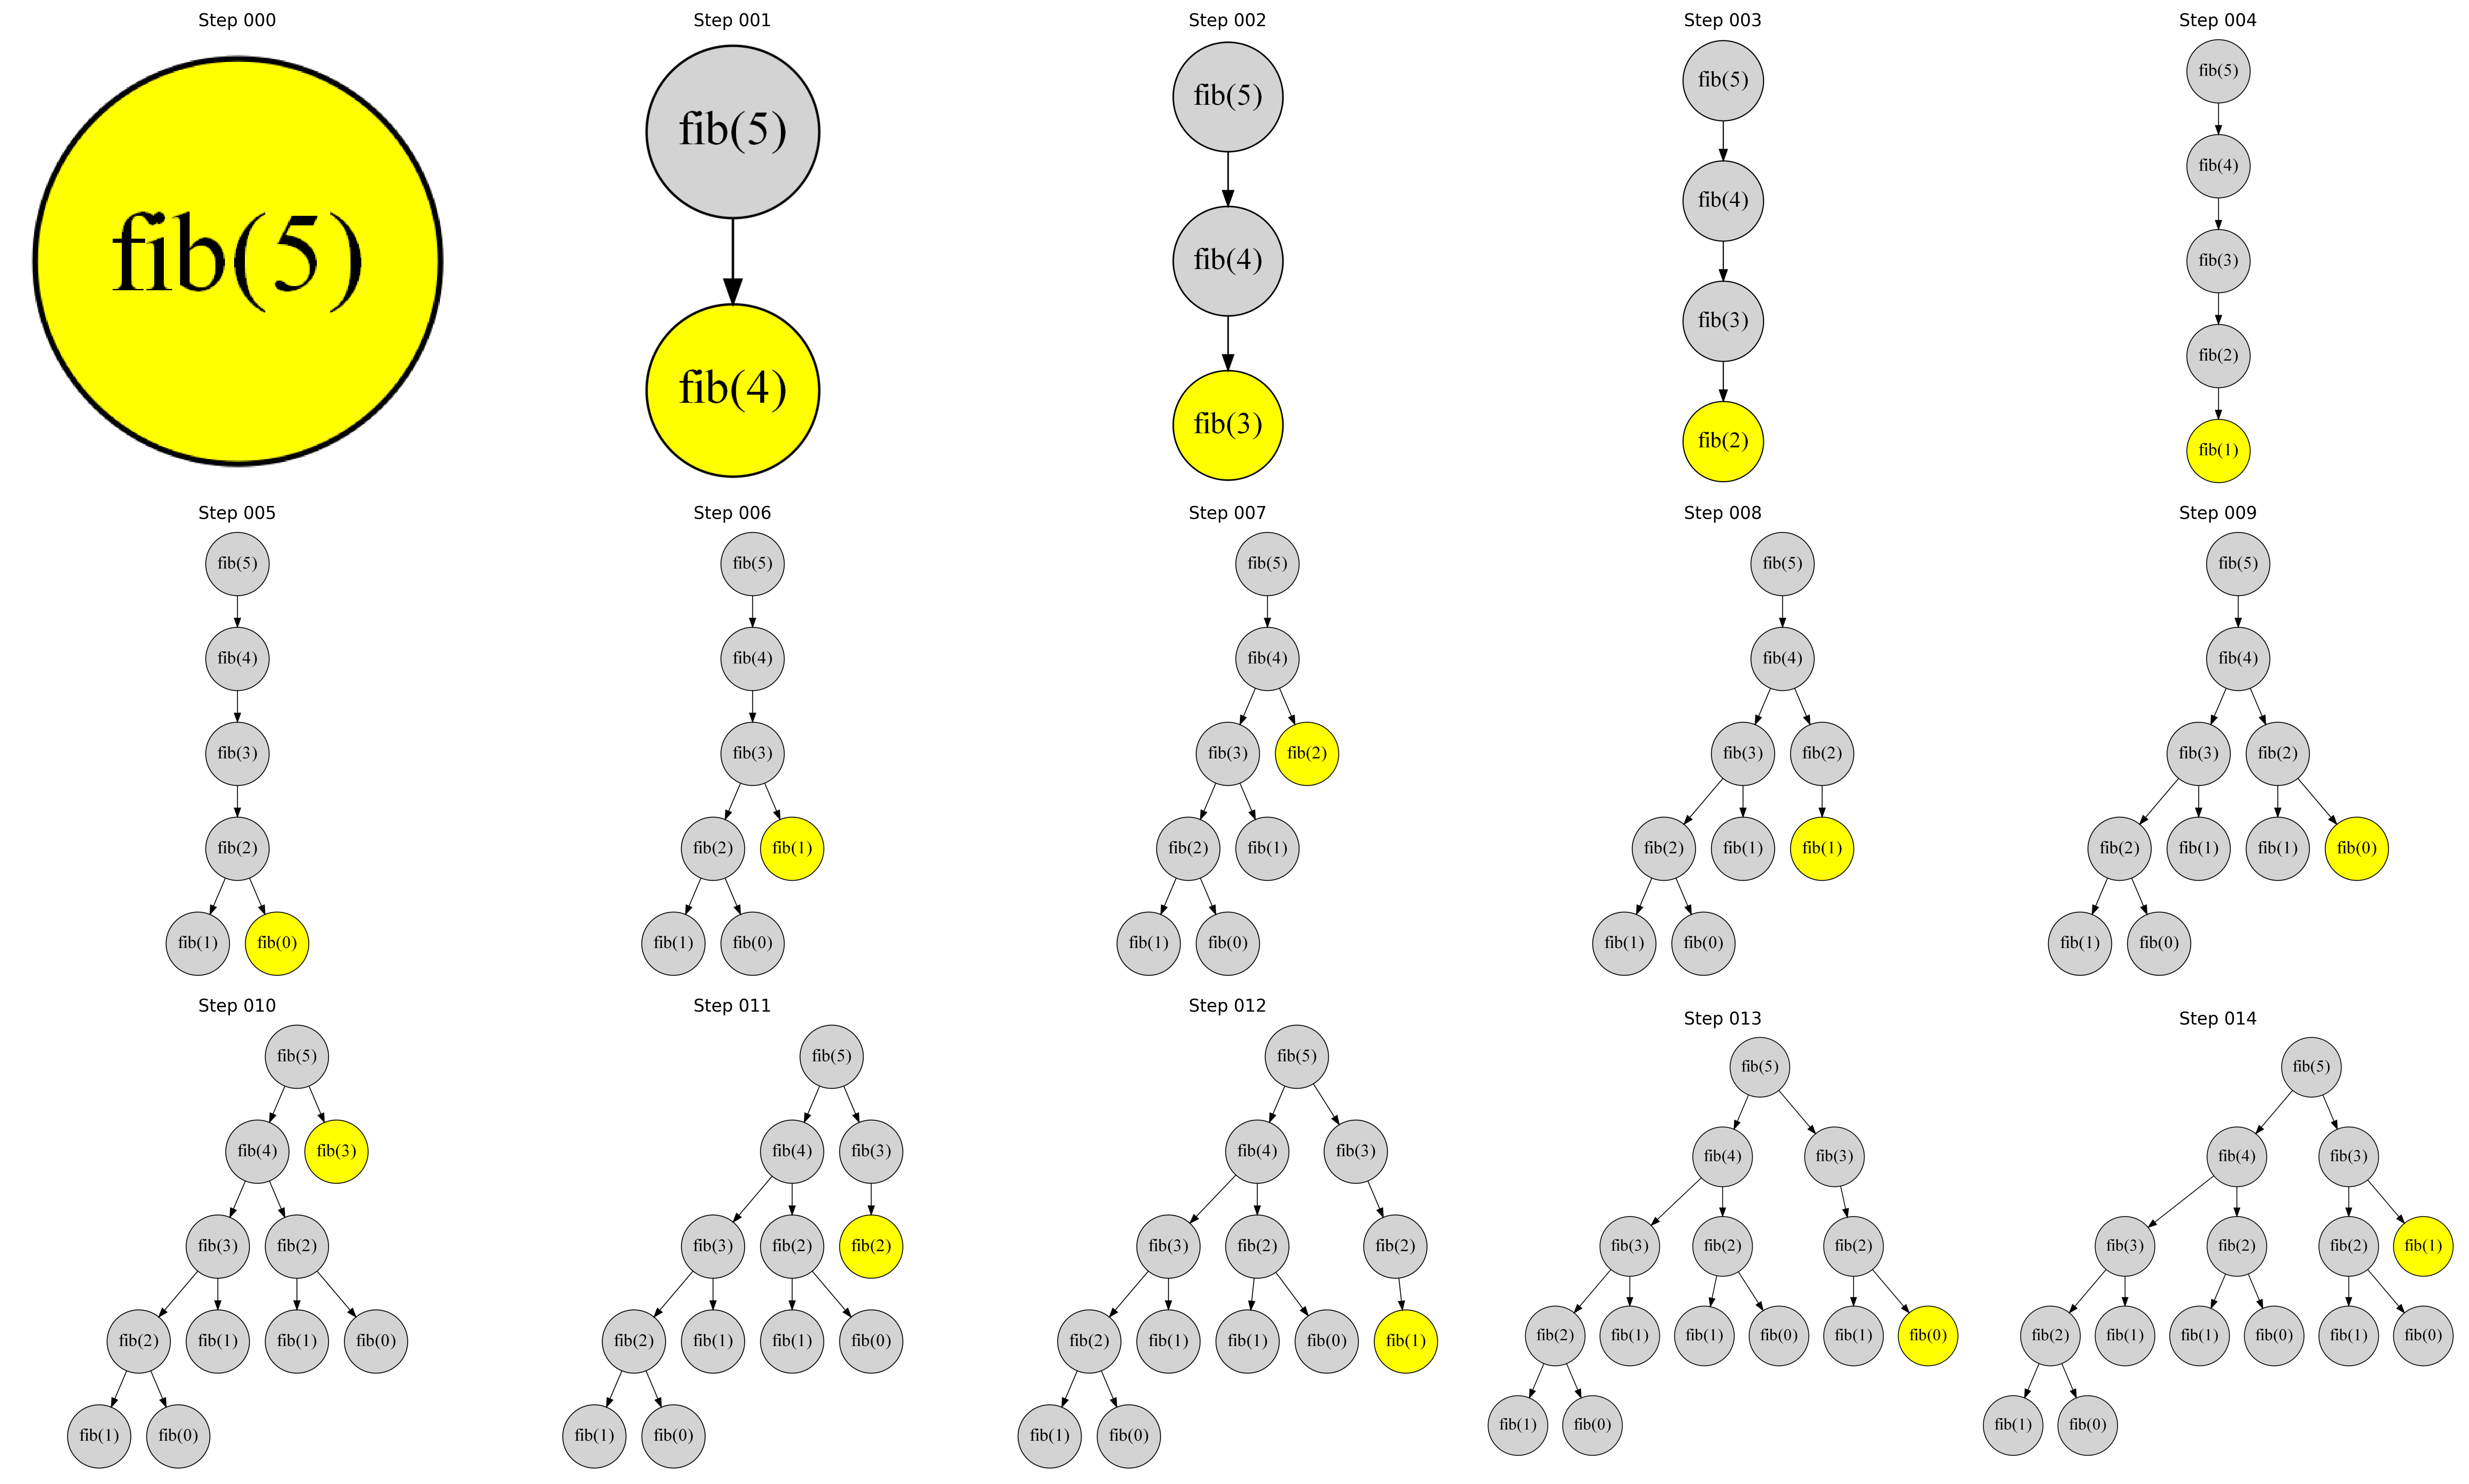
\includegraphics[width=0.9\textwidth]{./recursion-tree-animation/png/recursion_tree_combined.png}
	\caption{Recursion progress}
	\label{fig:fib_steps_progress}
\end{figure}

% Analyzing space complexity
\subsection{Space Complexity}
The space complexity is determined by the memory used on the call stack due to recursion. Although the recursion tree contains an exponential number of nodes (\( O(\phi^n) \)), not all nodes are active simultaneously. The call stack only holds the frames for the active recursive calls along a single path from the root to a leaf.

\subsubsection{Call Stack Analysis}
Consider the recursion tree for computing \( F(n) \). The deepest path in the tree occurs when the recursion follows \( F(n) \to F(n-1) \to F(n-2) \to \cdots \to F(0) \), which has a depth of \( n \). At any point, the call stack contains at most \( n \) frames, each storing a constant amount of data (e.g., the parameter \( n \) and return address).

For example:
- When computing \( F(n-1) \), the call for \( F(n-2) \) is not yet active.
- Once \( F(n-1) \) is resolved, its stack frame is popped, and \( F(n-2) \) is pushed onto the stack.

Thus, the maximum stack depth is \( n \), leading to a space complexity of:
\[
O(n).
\]

\subsubsection{Clarification on Exponential Misconception}
The total number of recursive calls is exponential, which might suggest exponential memory usage. However, since only one path of the recursion tree is active at a time, the call stack grows linearly with \( n \), not exponentially.

\subsection{JVM Debugger view}
\lstinputlisting[language=Java, caption={Minimal Debugger}]{./fibonacci-debugger/MinimalDebugger.java}
And target : 
\lstinputlisting[language=Java, caption={Debugger Target}]{./fibonacci-debugger/FibonacciTarget.java}
We should compile it with debugging info : 
\begin{lstlisting}[language=bash]
	javac -g -cp .;%JAVA_HOME%/lib/tools.jar *.java
\end{lstlisting}
To run app in debug mode we use this: 
\begin{lstlisting}[language=bash]
	java -cp .;%JAVA_HOME%/lib/tools.jar -agentlib:jdwp=transport=dt_socket,server=y,suspend=y,address=5005 FibonacciTarget
\end{lstlisting}
Then run debugger : 
\begin{lstlisting}[language=bash]
	java -cp .;%JAVA_HOME%/lib/tools.jar MinimalDebugger
\end{lstlisting}

Exploring debugger output : 
\lstinputlisting[language=bash, caption={Call frames in Java Debugger}]{./fibonacci-debugger/debugger-output.txt}

Debugger class diagram shown here

\begin{figure}[H]
	\centering
	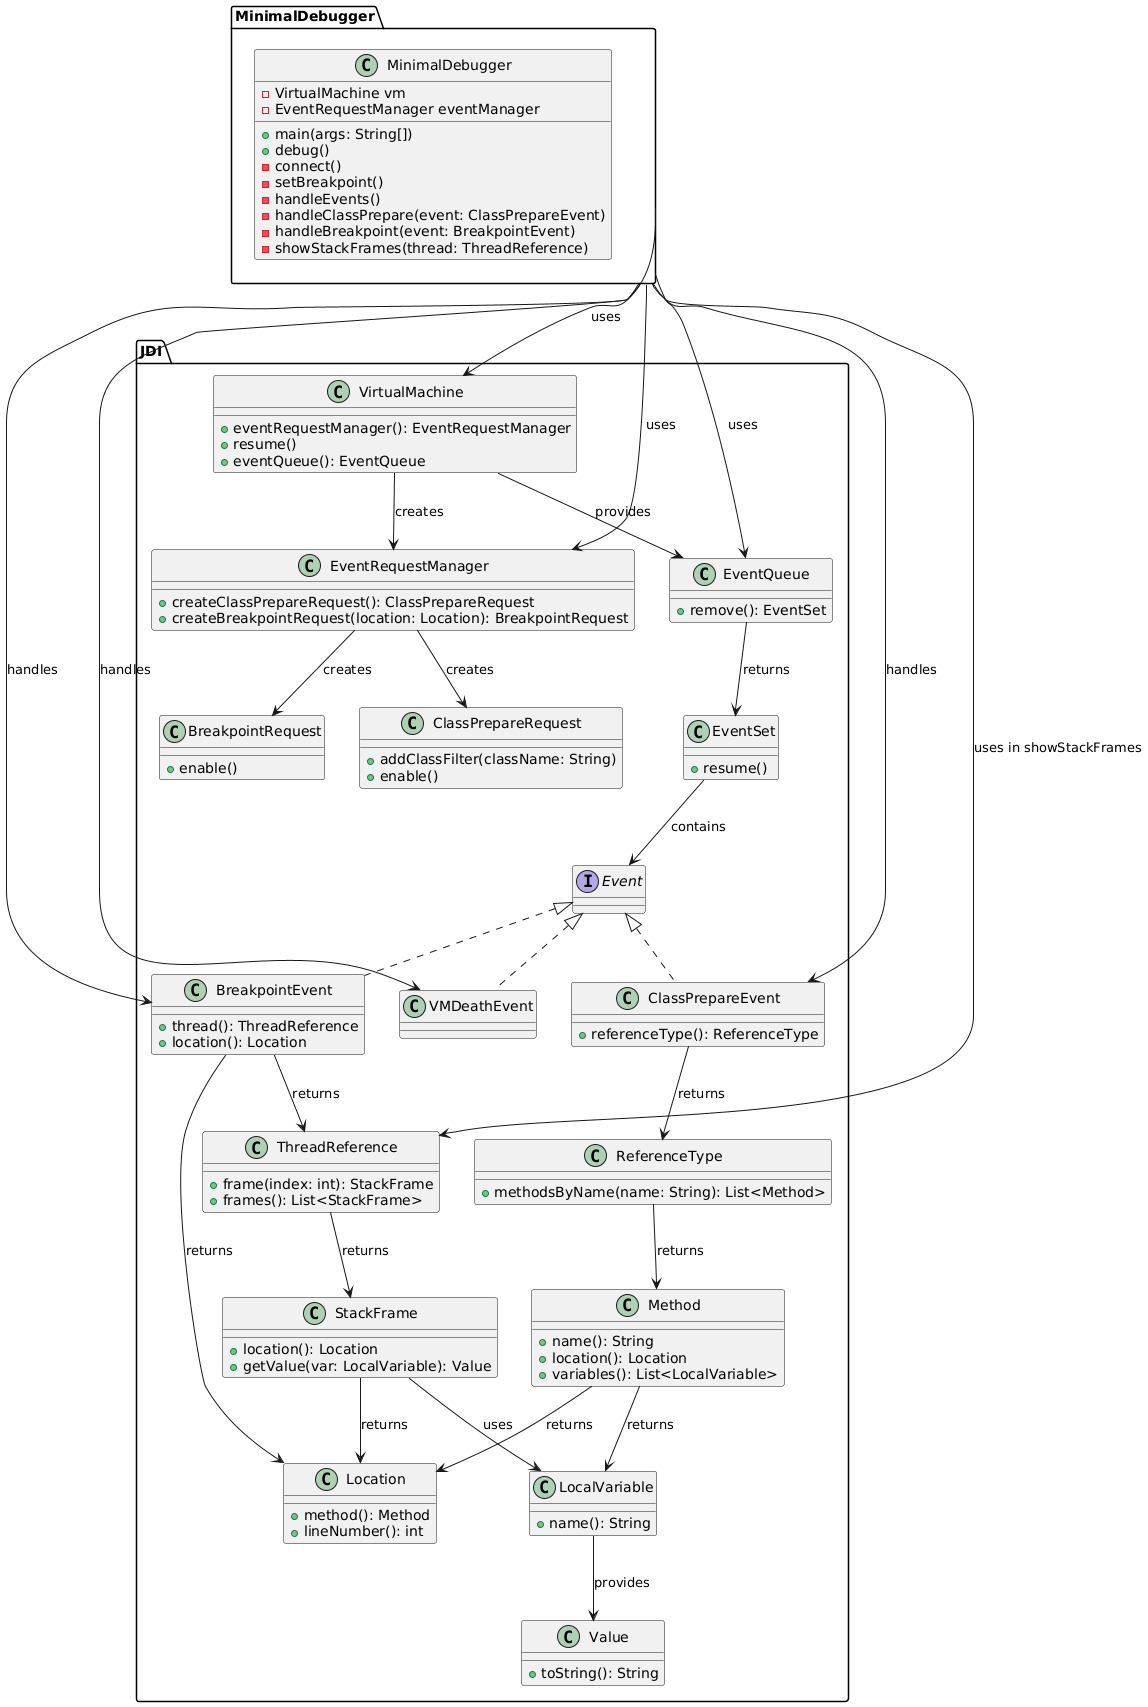
\includegraphics[width=0.9\textwidth]{./fibonacci-debugger/diagrams/class/DebuggerClass.png}
	\caption{Debugger class diagram}
	\label{fig:debugger_class_diagram}
\end{figure}


% Conclusion
\subsection{Conclusion}
The recursive Fibonacci algorithm has:
\begin{itemize}
	\item \textbf{Time Complexity}: \( O(\phi^n) \), where \( \phi \approx 1.618 \), due to the exponential number of nodes in the recursion tree.
	\item \textbf{Space Complexity}: \( O(n) \), due to the linear depth of the call stack, as only one path of the recursion tree is active at any time.
\end{itemize}

\section{Optimizing Recursion}
\subsection{Memoization}
Memoization stores computed values to avoid redundant calculations.

\lstinputlisting[language=Java,caption={Memoized Fibonacci}]{./optimizing-recursion/Memoization.java}

Time Complexity: $T(n) = \mathcal{O}(n)$ \\
Space Complexity: $M(n) = \mathcal{O}(n)$


\subsection{Dynamic Programming}
Dynamic programming (DP) avoids recursion entirely. We present two variants: array-based and space-optimized.
\lstinputlisting[language=Java,caption={Array-Based DP Fibonacci}]{./optimizing-recursion/ArrayDP.java}

\lstinputlisting[language=Java,caption={Space-Optimized DP Fibonacci}]{./optimizing-recursion/IterativeFibonacci.java}
Time Complexity: $T(n) = \mathcal{O}(n)$ \\
Space Complexity: $M(n) = \mathcal{O}(1)$ (optimized version)

\subsection{Linear algebra and Fibonacci}
\subsubsection{Matrices and Transformations}
We begin with the general concepts of matrices as linear transformations and matrix multiplication, then apply these ideas to the Fibonacci sequence, deriving its matrix form and geometric meaning.

Matrices represent linear transformations in vector spaces. A linear transformation \( T: \mathbb{R}^m \to \mathbb{R}^n \) preserves vector addition and scalar multiplication:
\[
T(\mathbf{u} + \mathbf{v}) = T(\mathbf{u}) + T(\mathbf{v}), \quad T(c \mathbf{u}) = c T(\mathbf{u}).
\]
For example, a 2x2 matrix defines a transformation \( T: \mathbb{R}^2 \to \mathbb{R}^2 \). Geometrically, such transformations can include rotations, scalings, shears, or reflections in the plane.

In the context of sequences like Fibonacci, we will use a specific matrix to model the recurrence as a linear transformation that iteratively evolves a state vector.

Matrix multiplication is defined such that the product \( AB \) represents the composition of the linear transformations corresponding to \( B \) followed by \( A \). For two matrices \( A \) (an \( m \times n \) matrix) and \( B \) (an \( n \times p \) matrix), the element \( (AB)_{ij} \) is the dot product of the \( i \)-th row of \( A \) and the \( j \)-th column of \( B \):
\[
(AB)_{ij} = \sum_{k=1}^n a_{ik} b_{kj}.
\]
This definition arises from the need to compose linear transformations. If \( T_A \) is the transformation for \( A \) and \( T_B \) for \( B \), then \( T_A(T_B(\mathbf{v})) = (AB) \mathbf{v} \).
Improve this def !!!

Geometrically, matrix multiplication corresponds to applying one transformation after another. For example, multiplying rotation matrices composes rotations; scaling followed by shearing distorts shapes accordingly. In sequences, repeated multiplication evolves the state over multiple steps, leading to growth or convergence patterns observable in geometric structures.

Building on linear transformations, we express the Fibonacci recurrence in matrix form. Represent a pair of consecutive Fibonacci numbers as a vector:
\[
\begin{bmatrix} F_n \\ F_{n-1} \end{bmatrix}.
\]
We seek a matrix \( A = \begin{bmatrix} a & b \\ c & d \end{bmatrix} \) such that:
\[
A \cdot \begin{bmatrix} F_n \\ F_{n-1} \end{bmatrix} = \begin{bmatrix} F_{n+1} \\ F_n \end{bmatrix}.
\]
Multiplying matrix to vector gives us the system of equations:
\begin{equation}
	\left\{
	\begin{aligned}
		a F_n + b F_{n-1} &= F_{n+1}\\
		c F_n + d F_{n-1} &= F_n
	\end{aligned}
	\right.
	\label{sys_fib}
\end{equation}

From the Fibonacci recurrence, we know:
\[
F_{n+1} = F_n + F_{n-1}.
\]
Comparing this with the first equation from system (\ref{sys_fib}), we get:
\[
a F_n + b F_{n-1} = F_n + F_{n-1}.
\]
For this to hold for all \( n \), the coefficients must match:
\[
a = 1, \quad b = 1.
\]
For second equation from (\ref{sys_fib}), we need:
\[
c F_n + d F_{n-1} = F_n.
\]
This implies:
\[
c = 1, \quad d = 0.
\]
Thus, the matrix is:
\[
A = \begin{bmatrix} 1 & 1 \\ 1 & 0 \end{bmatrix}.
\]
\\
This matrix acts as a linear transformation:
\[
A \begin{bmatrix} x \\ y \end{bmatrix} = \begin{bmatrix} x + y \\ x \end{bmatrix},
\]
which is a shear transformation. 

To find later terms, we use matrix powers:
\begin{equation}
	\begin{bmatrix} F_{n+1} \\ F_n \end{bmatrix} = \begin{bmatrix} 1 & 1 \\ 1 & 0 \end{bmatrix}^n \cdot \begin{bmatrix} 1 \\ 0 \end{bmatrix}
	\label{matrix_fib}
\end{equation}
This is what we were looking for - recurrence relation in matrix form for Fibonacci numbers. We'll visualize (\ref{matrix_fib}) later because it's fun.

\subsubsection{Algorithm implementation in Java}
\lstinputlisting[language=Java,caption={Fibonacci by Matrix exponentiation}]{./optimizing-recursion/MatrixFibonacci.java}

\subsubsection{Time and space complexity}
Time Complexity: $T(n) = \mathcal{O}(\log n)$ \\
Space Complexity: $M(n) = \mathcal{O}(1)$

\subsection{Computer Algebra Systems}
Using Maple, we can compute Fibonacci numbers efficiently:
\lstinputlisting[language=Maple,caption={Fibonacci in Maple}]{./optimizing-recursion/fibonacci.mpl}
Run with:
\begin{lstlisting}[language=bash,caption={Running Maple Script}]
cmaple -q fibonacci.mpl >out.log
\end{lstlisting}

\subsection{Binet formula in real life}

% Introducing the Binet formula and its theoretical complexity
The Binet formula provides a closed-form expression for the \(n\)-th Fibonacci number:
\[
F(n) = \frac{\phi^n - \psi^n}{\sqrt{5}},
\]
where \(\phi = \frac{1 + \sqrt{5}}{2}\) (the golden ratio) and \(\psi = \frac{1 - \sqrt{5}}{2}\). Since it directly computes \(F(n)\) without iterative steps, it has a theoretical time complexity of \(O(1)\) for a single computation, assuming arithmetic operations (like exponentiation) are constant-time. However, despite this apparent efficiency, the Binet formula is impractical for large \(n\) in computational practice for several reasons.

% Listing reasons for impracticality
\begin{enumerate}
	\item \textbf{Numerical Instability with Floating-Point Arithmetic}:
	For large \(n\), \(\phi^n\) grows exponentially, while \(\psi^n\) (with \(|\psi| < 1\)) becomes extremely small. Their difference, \(\phi^n - \psi^n\), involves subtracting two nearly equal values, leading to significant round-off errors in floating-point arithmetic (e.g., \texttt{double} in Java or C++). This causes inaccuracies, as seen when computing \(F(71)\), where floating-point results may deviate (e.g., 308061521170131 instead of the correct 308061521170129).
	
	\item \textbf{High Precision Requirements with Arbitrary-Precision Arithmetic}:
	To mitigate floating-point issues, arbitrary-precision arithmetic (e.g., \texttt{BigDecimal} in Java) can be used. However, computing \(\phi^n\), \(\psi^n\), and \(\sqrt{5}\) requires high precision (e.g., hundreds of decimal places for \(n \approx 100\)) to ensure the result is an exact integer after division by \(\sqrt{5}\). This significantly increases computational cost, as each operation (exponentiation, division) scales with the number of digits, making the effective time complexity much worse than \(O(1)\).
	
	\item \textbf{Computational Overhead of Irrational Numbers}:
	The Binet formula involves irrational numbers (\(\phi\), \(\psi\), \(\sqrt{5}\)), which are computationally expensive to handle with high precision. In contrast, iterative methods using integer arithmetic (e.g., with \texttt{BigInteger}) involve only simple additions, which are faster and inherently exact for Fibonacci numbers, as they are integers by definition.
	
	\item \textbf{Scalability Issues for Large \(n\)}:
	For very large \(n\) (e.g., \(n = 1000\)), the precision required for \(\sqrt{5}\) and \(\phi^n\) grows proportionally to \(n\), as the number of digits in \(F(n)\) is approximately \(n \cdot \log_{10}(\phi)\). This makes Binet's formula slower than iterative or matrix-based methods, which have logarithmic complexity (\(O(\log n)\) with fast exponentiation) but operate on integers.
	
	\item \textbf{Implementation Complexity}:
	Implementing Binet's formula requires careful management of precision and rounding to ensure integer results, which adds complexity compared to the straightforward iterative approach (e.g., \(F(n) = F(n-1) + F(n-2)\)). The latter is simpler to code and debug, as it avoids dealing with floating-point or arbitrary-precision libraries.
\end{enumerate}

% Concluding with a comparison to iterative methods
In conclusion, while the Binet formula is theoretically \(O(1)\), its practical performance is hindered by numerical instability, high precision requirements, and computational overhead for irrational numbers. Iterative methods, or matrix exponentiation methods with \(O(\log n)\) complexity, are preferred in practice due to their simplicity, exactness, and efficiency, especially for large \(n\). For example, computing \(F(71)\) iteratively with \texttt{BigInteger} is faster and guarantees the correct result (308061521170129) without precision management.


\subsection{Conclusion}
We explored Fibonacci computation methods, from naive recursion ($\mathcal{O}(2^n)$) to matrix exponentiation ($\mathcal{O}(\log n)$). Below is a comparison:

\begin{table}[h]
	\centering
	\begin{tabular}{|l|c|c|}
		\hline
		\textbf{Method} & \textbf{Time Complexity} & \textbf{Space Complexity} \\
		\hline
		Naive Recursion & $\mathcal{O}(2^n)$ & $\mathcal{O}(n)$ \\
		Memoization & $\mathcal{O}(n)$ & $\mathcal{O}(n)$ \\
		Dynamic Programming & $\mathcal{O}(n)$ & $\mathcal{O}(1)$ \\
		Binet's Formula & $\mathcal{O}(1)$ & $\mathcal{O}(1)$ \\
		Matrix Exponentiation & $\mathcal{O}(\log n)$ & $\mathcal{O}(1)$ \\
		\hline
	\end{tabular}
	\caption{Complexity Comparison of Fibonacci Methods}
\end{table}

For large $n$, matrix exponentiation or BigDecimal-based DP are recommended. Future exploration could include fast doubling algorithms or parallel computation.

\section{Limitations of Primitive Types for Large Fibonacci Numbers}
\subsection{Showcase : from int to double}
\lstinputlisting[language=Java]{./data-types-limitations/LargestExactFibonacci.java}
\subsection{When double goes wild}
\subsubsection{$0.1 + 0.2 \ne 0.3$}
In Java, when running the program
\begin{lstlisting}[language=Java]
	public class A {
		public static void main(String[] args) {
			double x = 0.1;
			double y = 0.2;
			double z = x + y;
			System.out.println(z);
		}
	}
\end{lstlisting}
the output is
\begin{verbatim}
	0.30000000000000004
\end{verbatim}
instead of exactly \texttt{0.3}. \\

If you think Java is broken, try it in JavaScript or Python\\
JS:
\begin{lstlisting}[language=C++]
const x = 0.1;
const y = 0.2;
const z = x + y;
console.log(z);
\end{lstlisting}
Python:
\begin{lstlisting}[language=Python]
x = 0.1
y = 0.2
z = x + y
print(z)
\end{lstlisting}

Output : 
\begin{lstlisting}[language=bash]
C:\temp\>java A
0.30000000000000004

C:\temp\>node a.js
0.30000000000000004

C:\temp\>python a.py
0.30000000000000004	
\end{lstlisting}

This behavior is not a bug, but a direct consequence of the \emph{IEEE 754 double-precision floating-point format}.

\subsubsection{IEEE 754 Representation}
A Java \texttt{double} uses 64 bits:
\begin{itemize}
	\item 1 bit for the \emph{sign},
	\item 11 bits for the \emph{exponent},
	\item 52 bits for the \emph{mantissa} (fraction).
\end{itemize}

The value is computed as
\[
(-1)^{\text{sign}} \times 1.\text{mantissa} \times 2^{(\text{exponent} - 1023)}.
\]

\subsubsection{Calculate as machines}
The decimal fraction $0.1 = \tfrac{1}{10}$ has no finite binary expansion.
In base 2 it becomes
\[
0.1_{10} = 0.00011001100110011\ldots_2
\]
with repeating pattern \texttt{0011}. Since only 52 bits are available for
the mantissa, this value is stored approximately as
\[
0.10000000000000000555\ldots
\]

Similarly,
\[
0.2 \approx 0.2000000000000000111, \quad
0.3 \approx 0.2999999999999999889.
\]
Therefore,
\[
0.1 + 0.2 \approx 0.3000000000000000444,
\]
which is printed as \texttt{0.30000000000000004}.
\\
The decimal system can exactly represent fractions like $1/10$ or $1/5$,
but binary cannot. Binary floating-point can exactly represent only fractions
whose denominators are powers of two (e.g., $1/2$, $1/4$, $1/8$). Numbers like
$1/10$ or $1/5$ become infinite binary fractions, which must be rounded.

\subsubsection{Conclusion}
The result \texttt{0.30000000000000004} is not an error, but the inevitable
effect of representing decimal fractions in binary with limited precision.
Understanding IEEE 754 is essential for writing correct numerical programs.

\subsection{Handling Large Numbers with BigDecimal}
The \texttt{int} and \texttt{long} types in Java overflow for large Fibonacci numbers (e.g., $F_{93}$ exceeds \texttt{long}). We use \texttt{BigDecimal} for arbitrary-precision arithmetic to address this limitation.

\begin{lstlisting}[caption={Fibonacci with BigDecimal}]
import java.math.BigDecimal;

public static BigDecimal fibBigDecimal(int n) {
    if (n <= 0) return BigDecimal.ZERO;
    if (n == 1) return BigDecimal.ONE;
    
    BigDecimal prev = BigDecimal.ZERO;
    BigDecimal curr = BigDecimal.ONE;
    for (int i = 2; i <= n; i++) {
        BigDecimal next = prev.add(curr);
        prev = curr;
        curr = next;
    }
    return curr;
}
\end{lstlisting}

Time Complexity: $T(n) = \mathcal{O}(n \cdot M)$, where $M$ is the cost of BigDecimal operations. \\
Space Complexity: $M(n) = \mathcal{O}(1)$

\section{Real-World Applications}
\subsection{Fibonacci heaps for Dijkstra's algorithm optimization}
bla-bla-bla
\subsection{Fibonacci retracement levels in stock market analysis}
bla-bla-bla
\subsection{Some of pseudorandom number generators}
bla-bla-bla


\begin{thebibliography}{9}
\bibitem{knuth}
Knuth, D. E. (1997). \textit{The Art of Computer Programming, Volume 1: Fundamental Algorithms}. Addison-Wesley.
\bibitem{maple}
MapleSoft. (2025). Fibonacci Function Documentation. \url{https://www.maplesoft.com/support/help/Maple/view.aspx?path=combinat/fibonacci}.
\bibitem{wiki}
Wikipedia. (2025). Fibonacci Number. \url{https://en.wikipedia.org/wiki/Fibonacci_number}.
\bibitem{curve_fit}
SciPy docs \url{https://docs.scipy.org/doc/scipy/reference/generated/scipy.optimize.curve_fit.html}
\end{thebibliography}

\end{document}
